% Preamble
% ******************
\documentclass[a4paper,12pt]{report}
% margin
\usepackage[margin=2.5cm]{geometry}
% line spacing
\setlength{\parindent}{4em}
\setlength{\parskip}{1em}
\renewcommand{\baselinestretch}{1.5}
% citation
\usepackage{cite}
% Subfolders
\usepackage{subfiles}
% Graphics
\usepackage{subcaption} % Note: Subcaption and subfig are alternatives
% \usepackage{subfig}
\usepackage{graphicx}
\usepackage{placeins} % For float barriers
\graphicspath{{res/}{../res/}} % path variable for graphics folders
% other
\usepackage[utf8]{inputenc}
\usepackage{amsmath}
\usepackage{amsfonts}
\usepackage{amssymb}
\usepackage{hyperref}


% ******************
% \title{A review of semantic segmentation, vision transformers and domain adaptation}
% \author{Moritz Bergemann - 19759948}
% ******************



% ******************
\begin{document}{}
\begin{titlepage}
    \begin{center}
        \vspace*{0.5cm}
            
        \LARGE
        \textbf{A Review of Semantic Segmentation, Vision Transformers and Domain Adaptation}
            
        % \vspace{0.3cm}
        % Utilising 
            
        \vspace{1.0cm}
        \Large
            
        \textbf{Moritz Bergemann\\ 19759948}
            
        \vfill
            
        Literature Review
            
        \vspace{2.5cm}
            
        % \includegraphics[width=0.4\textwidth]{university}
            
        \large
        School of Electrical Engineering, Computing and Mathematical Sciences\\
        Curtin University\\
        Australia\\
        June 2022
            
    \end{center}
\end{titlepage}

\newpage
\tableofcontents
\newpage
\listoffigures
\newpage
\listoftables
\newpage
\thispagestyle{empty}

% BEGIN CONTENT
\chapter{Literature Review}
    \section{Semantic segmentation}
    Semantic segmentation is a core task in computer vision that involves performing classification on every pixel in an input image. Unlike other computer vision tasks such as image classification (identifying which of a set of classes an input image belongs to) or object detection (identifying, classifying, and locating objects in an image), semantic segmentation provides highly dense and semantically rich information, particularly about the shapes objects take up and the intersections between objects.
    
    \begin{figure}[h]
        \centering
        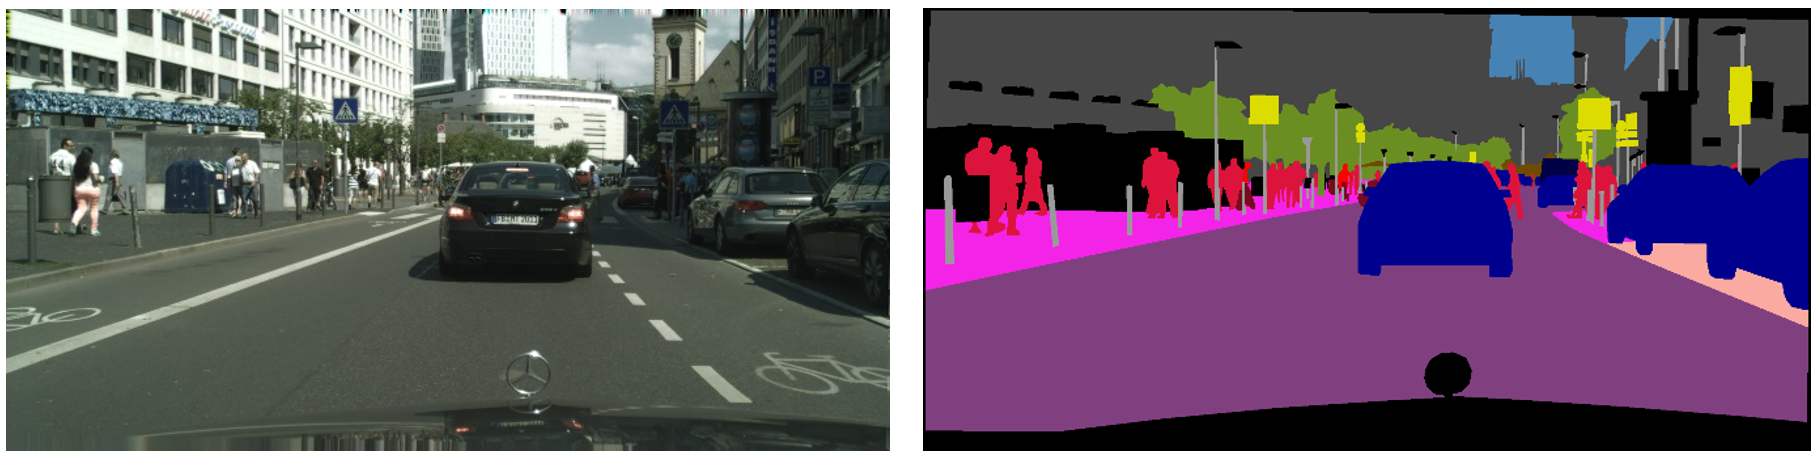
\includegraphics[width=\textwidth]{res/cityscapes-segmentation-sample.png}
        \caption{An example of an annotated semantic segmentation image from the Cityscapes dataset \cite{cordts_cityscapes_2016}. The left is the input to the model, and the right is the expected output.}
        \label{fig:convolution}
    \end{figure}
    
    Segmentation is a key pre-processing task for many applications. Use in self-driving cars and robotics is most often cited. To safely drive, a self-driving car must be able to identify the shape, course, and edges of the road in front of it rather than only identifying it as a road, for instance. Medical analysis is another key segmentation task that can helps automate the essential task of medical identification and analysis. Many publications focus exclusively on the segmentation of CT or MRI images for medical applications \cite{hesamian_deep_2019}. Other applications include satellite mapping, video surveillance, augmented reality, and domain transformation \cite{richter_enhancing_2021}.
    
    Semantic segmentation is distinguished from other computer vision tasks through its density and computational complexity. Density is key in segmentation as the output is pixel-wise - therefore, a significant amount of information must be known about each pixel in the image to accurately segment it, especially for the boundaries between images. The increase in computational cost is also intuitive. No matter the scenario, generating an output that has the same dimensions as the model input will be more computationally intensive than a classification model that simply outputs a single vector.
    
    As with most computer vision applications, deep convolutional neural networks (CNNs) have traditionally achieved state-of-the-art results on semantic segmentation tasks for accuracy and efficiency. The superior performance of CNNs is often cited to be due to their possession of vision-specific inductive biases. Translational equivariance means that patterns present anywhere in an image will be extracted in the same way due to the constant convolution kernel that “slides” across the input. Locality means that CNNs, due to the limited size of each kernel, will inherently put stronger weights towards input features that are closer together in 2D space (figure ~\ref{fig:receptive_field}) \cite{zhang_dive_2019}. All of this is achieved with fixed-size kernels, meaning the number of parameters that must be trained for any model does not increase with image size. Novel advances in general computer vision are typically first made on the simpler image classification task, then transferred to other tasks like segmentation.
    
    \begin{figure}[ht]
        \centering
        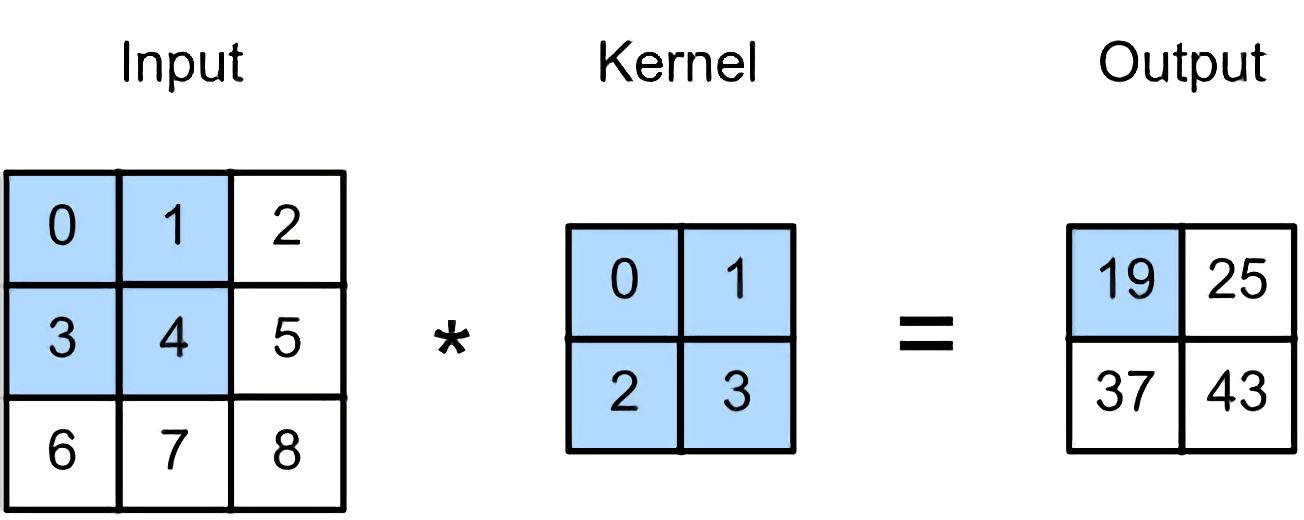
\includegraphics[scale=0.7]{res/convolution.png}
        \caption{A single step in the 2D convolution of an input tensor with a kernel \cite{zhang_dive_2019}. The next stage would be the computation of $25$ via $1 \times 0 + 2 \times 1 + 4 \times 2 + 5 \times 3$.}
        \label{fig:convolution}
    \end{figure}

    \begin{figure}
        \centering
        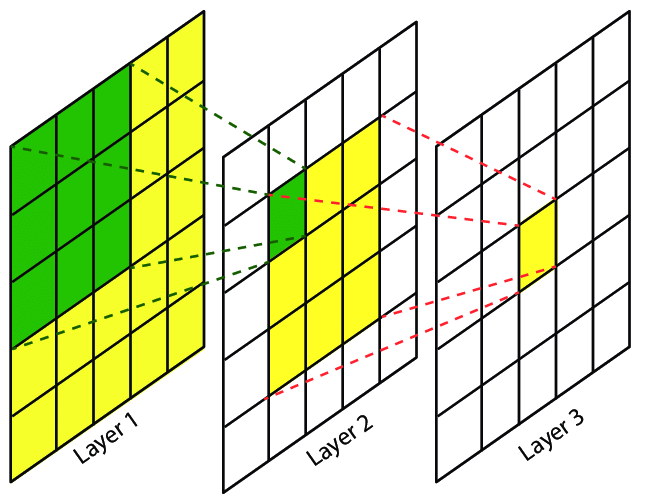
\includegraphics[scale=0.3]{res/receptive-field.png}
        \caption{A visualisation of locality across CNN layers \cite{lin_maritime_2017} - the neuron in each layer is only defined by the spatially close neurons in the previous layer. This is also demonstrates CNNs' limited receptive field.}
        \label{fig:receptive_field}
    \end{figure}
    
    Many initial segmentation approaches used CNNs in a multi-stage process, applying them only for some components. \cite{gupta_learning_2014} use CNNs as the feature extractor, to which an SVM is applied for region proposal, followed by decision trees for segmentation. R-CNN \cite{girshick_rich_2014} uses traditional machine learning approaches to first compute region proposals which are then passed through a CNN for classification or segmentation. However, the majority of recent publications find more success using an end-to-end approaches that can be trained via a single back-propagation pass.
    
    FCN (Fully Convolutional Network) \cite{long_fully_2015} was the first model to introduce the concept of using state-of-the-art deep classification networks as “backbones” for segmentation models. The classification models (commonly VGGNet \cite{simonyan_very_2015}, ResNet \cite{he_deep_2015}, or Xception \cite{chollet_xception_2017} in convolutional models) are modified to act as feature extractors, retrieving high-level representations of the input image which can then be used for segmentation rather than classification. This approach, common in many state-of-the-art segmentation models, takes advantage of the backbone's proven architectures and their strong feature extraction abilities due to pre-training on much larger classification datasets such as ImageNet \cite{russakovsky_imagenet_2015}, or more recently JFT \cite{sun_revisiting_2017}. Though state-of-the-art, FCN struggled with the learning of global context and with feature localisation (important for dense prediction). These issues were addressed in early approaches through global pooling \cite{liu_parsenet_2015} and conditional random fields \cite{chen_semantic_2016}.
    
    Most semantic segmentation approaches follow some kind of encoder-decoder structure \cite{zhang_dive_2019}. Common in many image-to-image and sequence-to-sequence deep learning tasks, this approach consists of two parts. The encoder first maps the input sequence to an abstract representation, typically known as a feature space. The backbones introduced in FCN may be considered encoders, for instance. The decoder is the second component, which reconstructs an output image from this representation (in this case a segmentation map). U-Net \cite{ronneberger_u-net_2015}, ubiquitous in medical segmentation applications, is an early example of a backbone-less encoder-decoder for segmentation.
    
    \begin{figure}[ht]
        \centering
        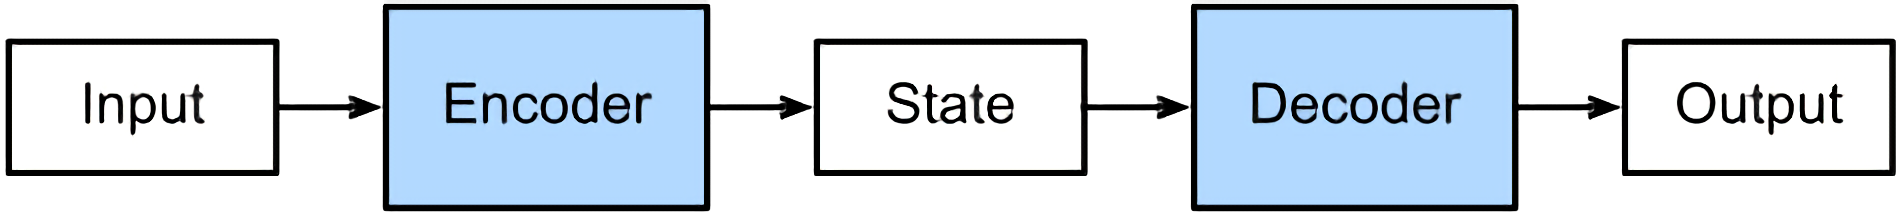
\includegraphics[width=\textwidth]{res/encoder-decoder.png}
        \caption{The encoder-decoder architecture \cite{zhang_dive_2019}.}
        \label{fig:encoder_decoder}
    \end{figure}
    
    Extraction of features at multiple scales is also important for dense prediction - a car in the distance will be differently sized to a car in the foreground, but both should be labelled accurately. This can be addressed by feeding in and parsing inputs at multiple scales, as in RefineNet \cite{lin_refinenet_2016} or using multi-scale pooling techniques. \cite{he_spatial_2014} introduced the Spatial Pyramid Pooling (SPP) module, which pools input features to multiple resolutions and then applies convolutions to the output to produce a multi-scale feature vector. PSPNet \cite{zhao_pyramid_2017} applied this approach to semantic segmentation by producing, upsampling, and then appending the multi-scale feature maps while maintaining shape (figure ~\ref{fig:pspnet_architecture}) to produce segmentation results.
    
    \begin{figure}[hb]
        \centering
        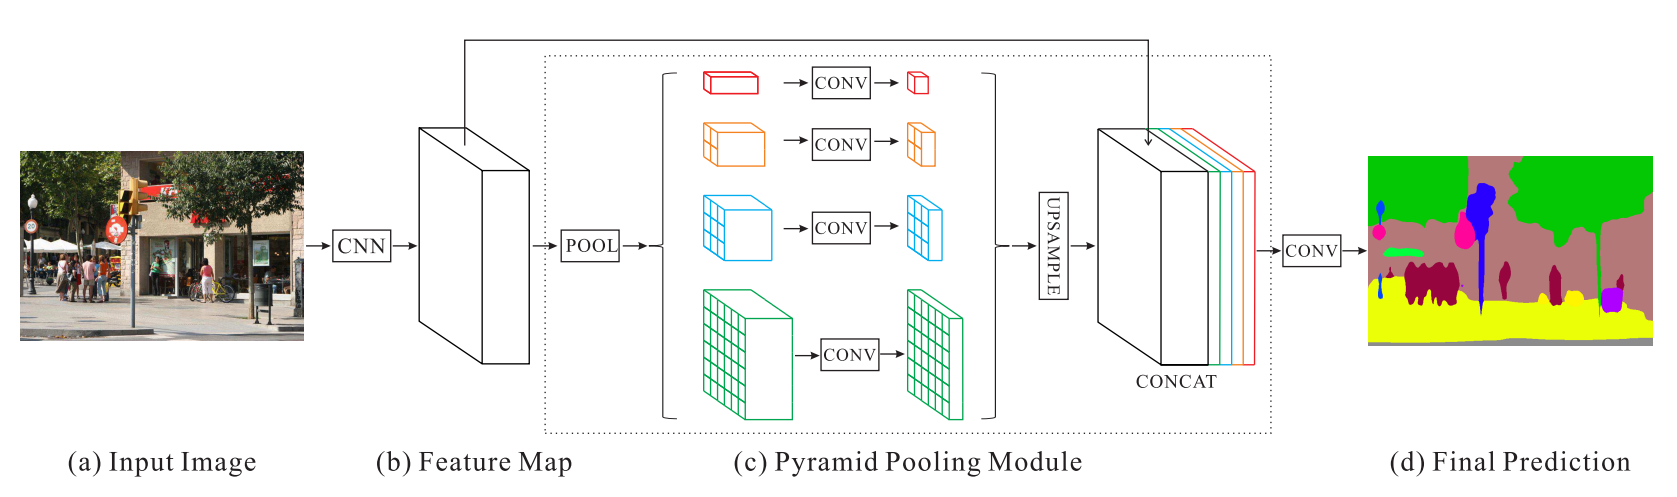
\includegraphics[width=\textwidth]{res/pspnet-architecture.png}
        \caption{Architecture of PSPNet's Pyramid Pooling Module \cite{zhao_pyramid_2017}, which extracts features at multiple scales.}
        \label{fig:pspnet_architecture}
    \end{figure}

    In recent years, the DeepLab series of models have set the baseline for efficient and performant semantic segmentation. DeepLab \cite{chen_semantic_2016} introduced the atrous convolution for dense prediction tasks. Atrous convolutions introduce gaps between the weights used to inform the next layer’s pixels, allowing for a larger receptive field without significantly increasing model parameters. DeepLabV2 \cite{chen_deeplab_2017} builds on this via Atrous Spatial Pyramid Pooling (ASPP), which combines PSPNet’s \cite{zhao_pyramid_2017} multi-scale features with awider receptive field (figure ~\ref{fig:deeplab_aspp}). DeeplabV3 \cite{chen_rethinking_2017} introduces a deeper architecture and adds a resizing component to ASPP that better suits atrous convolution’s large receptive field. DeepLabV3+ \cite{chen_encoder-decoder_2018} introduced an encoder-decoder design with DeepLabV3 as the encoder, and applies a simple decoder to better refine class boundaries. DeeplabV3+ achieves 82.1\% mIoU on the Cityscapes dataset \cite{cordts_cityscapes_2016}, a common benchmark for segmentation models.
    
    \begin{figure}[t]
        \centering
        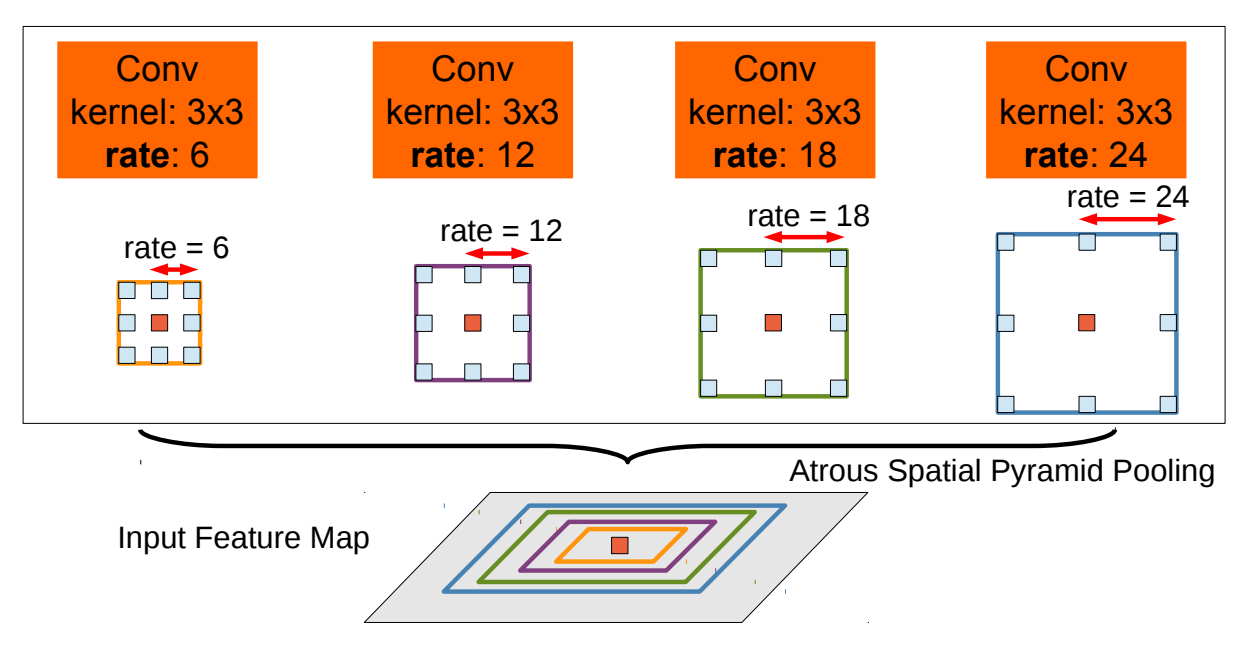
\includegraphics[scale=0.5]{res/deeplab-aspp.png}
        \caption{Visualisation of atrous spatial pyramid pooling \cite{chen_deeplab_2017}.}
        \label{fig:deeplab_aspp}
    \end{figure}
    
    \subsection{Fast semantic segmentation}
    The density and number of predictions (typically one per input pixel) required for semantic segmentation makes it one of the most computationally expensive computer vision tasks. The large number of predictions in the output layer itself is computationally expensive, but dense predictions also typically require a higher-resolution feature map, further increasing memory and compute requirements. Many state-of-the-art segmentation models are therefore only capable of running at a speed of 2-3 predictions a second on modern hardware \cite{zhao_icnet_2018}. Since many uses of segmentation, such as self-driving cars and robotics, require segmentation to be performed in real-time, extensive research has been done to improve the efficiency of semantic segmentation. 
    
    ENet (Efficient Net) \cite{paszke_enet_2016} was one of the first models to explore low-resource segmentation, focusing on reasonable accuracy capable of running in real-time on mobile devices. It achieves this by making select sacrifices to minimise model parameters and computations while mitigating drops in accuracy. Input features are quickly downsampled to a low resolution ($\frac{1}{8}$th input) with a small number of features, as minimising information density early in the model (forcing the model to “compress” image information) was found to only minimally reduce performance. The model also minimises the size of the decoder, and employs atrous and factorised convolutions to increase receptive field without increasing computation. E-Net achieves 58.3\% mIoU on the Cityscapes test set with 0.37M parameters, compared to the then state-of-the art DeepLab’s 63.1\% mIoU with 134.3M parameters.

    \begin{figure}[t]
        \centering
        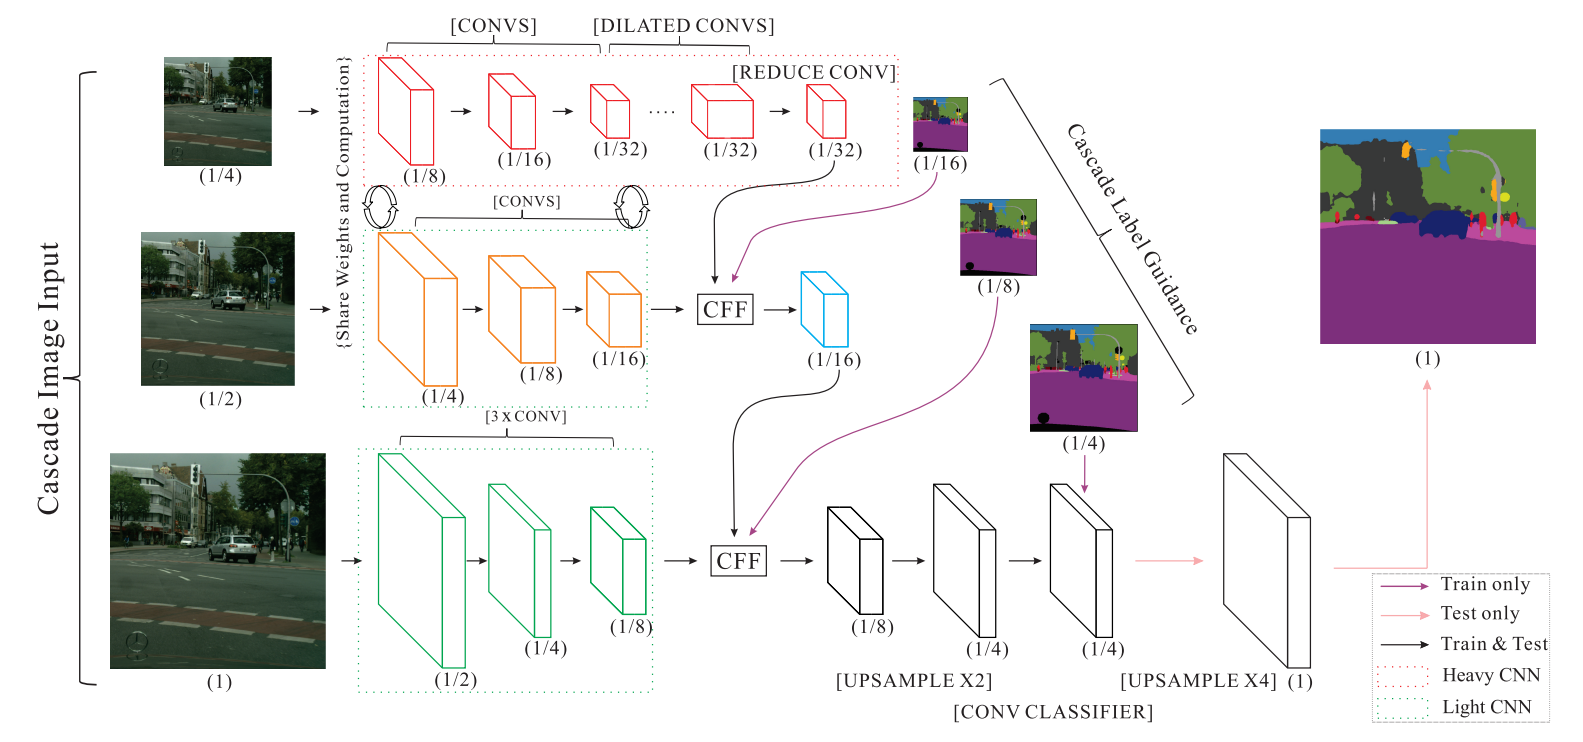
\includegraphics[width=\textwidth]{res/icnet-architecture.png}
        \caption{ICNet architecture \cite{zhao_icnet_2018}.}
        \label{fig:icnet_architecture}
    \end{figure}

    ICNet (Image Cascade Network) \cite{zhao_icnet_2018} in 2018 was the next major model to tackle the fast segmentation problem. Initial approaches had an inherent trade-off: reduced input size increases speed, as less convolutions must be performed, but reduces segmentation accuracy, as there are less fine details. ICNet addresses this by taking in the same input image at different scales. High-resolution inputs are parsed through low-filter-count layers that are lightweight but still capable of extracting low-level details like edge and texture. Low-resolution inputs are parsed through more expensive high-filter-count layers capable of extracting high-level object information (e.g. “these pixels represent a car”), where the low resolution keeps computation time low. The computed features are then fused together through multiple “cascades” to produce the final features. This approach - delegating high-resolution branches to low-level details and vice versa - has become a staple of fast segmentation. BiSeNet \cite{yu_bisenet_2018} extends ICNet’s multi-resolution approach, finding that two ‘branches’, one high-resolution (the “spatial path”) and one low resolution (the “context path”) is most effective.
    
    Many efficient segmentation models rely on innovations from other computer vision domains. The MobileNet \cite{howard_mobilenets_2017} classification models introduced the depthwise separable convolution block, which splits a standard convolution into a (far less expensive) combination of pointwise and depthwise convolution with minimal accuracy loss. MobileNetV2 \cite{sandler_mobilenetv2_2019} introduces the bottleneck residual block, which performs efficient convolutions by transforming inputs into a high-dimensional manifold. ContextNet \cite{poudel_contextnet_2018} uses a two-branch architecture like BiSeNet \cite{yu_bisenet_2018}, and introduces depthwise separable convolutions and bottleneck residual blocks for the high (shallow) and low (deep) resolution branches respectively. ContextNet’s successor, Fast-SCNN \cite{poudel_fast-scnn_2019}, has become a benchmark for fast segmentation performance. Fast-SCNN replaces the high-resolution branch with a “learning-to-downsample” module that downsamples the input, learns simple high-resolution features, and is used as input to the deep branch. The shallow high-resolution information is then simply fed into the final output features via a skip-connection (figure ~\ref{fig:fastscnn_architecture})
    
    \begin{figure}[h]
        \centering
        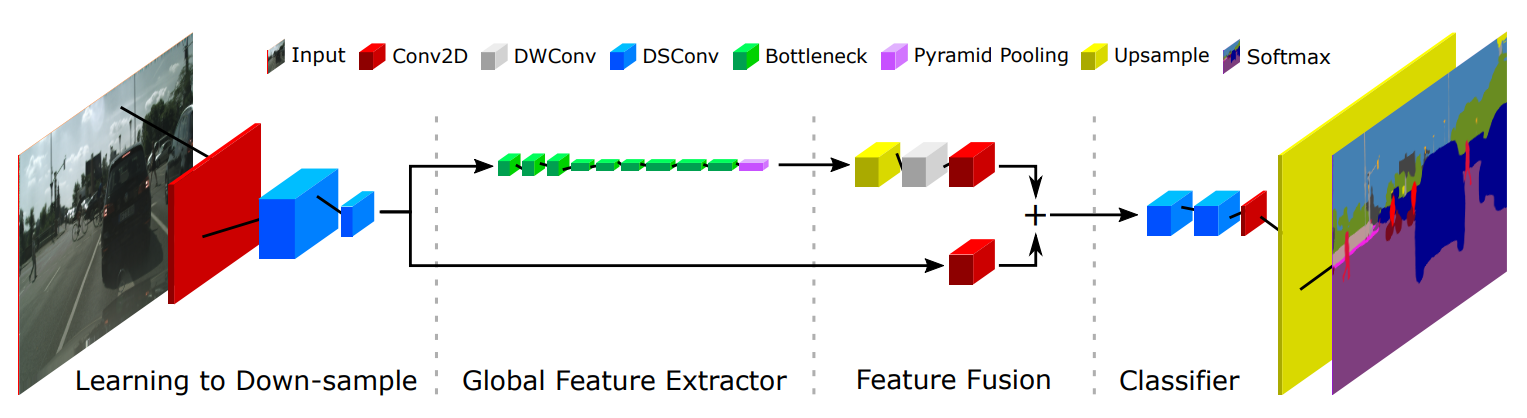
\includegraphics[width=\textwidth]{res/fastscnn-architecture.png}
        \caption{Fast-SCNN architecture \cite{poudel_fast-scnn_2019}.}
        \label{fig:fastscnn_architecture}
    \end{figure}
    
    \subsection{Transformers for semantic segmentation}
    
    The transformer architecture revolutionised the deep learning field in 2017 \cite{vaswani_attention_2017}. Initially applied for sequence-based natural language processing (NLP) tasks, transformers propose a fundamentally different approach to CNNs. Transformers are based on the concept of multi-head attention. Given two sequences $A$ and $B$ (sequences of words in the initial paper), attention computes the importance of each element in one sequence to each element in the other. This is done by retrieving a query $Q$ from $B$, and a key $K$ and value $V$ from $B$ - all computed through trainable linear layers. Self-attention then effectively applies a mask to $V$ based on the importance between $Q$ and $K$. Self-attention is an instance of this where $Q$, $K$, and $V$ are computed from the same input, meaning the computed mask defines the importance between each item in the input sequence. “Multi-Head” implies this process is performed multiple times with different linear layers to compute $Q$, $K$, and $V$, similarly to having multiple filters for different features in CNNs.
    
    In the same way that sentences can be considered an ordered sequence of words, an image could be considered an ordered sequence of pixels for use with a transformer (figure ~\ref{fig:vit_attention}). While various works have explored the integration of self-attention into CNN-based architectures, ViT \cite{dosovitskiy_image_2021} was the first attempt to produce a fully transformer-based vision architecture (as in \cite{vaswani_attention_2017}) modified for image inputs. Rather than encoding each pixel into the input sequence (which would be prohibitively expensive), ViT groups the input image into $16 \times 16$ patches for encoding into the input sequence. Transformers became ubiquitous in NLP due to their ability to map long-distance relationships and their extreme scalability with increasing amounts of data \cite{devlin_bert_2019} \cite{radford_language_2019}. However, transformers lack the translational equivariance and locality that are believed to make CNNs so effective for vision, and experiments indeed showed that ViT is outperformed by state-of-the-art CNNs when trained on smaller datasets. However, when trained on extremely large datasets, the scalability of transformers appears to win out against these biases.
    
    \begin{figure}[h]
        \centering
        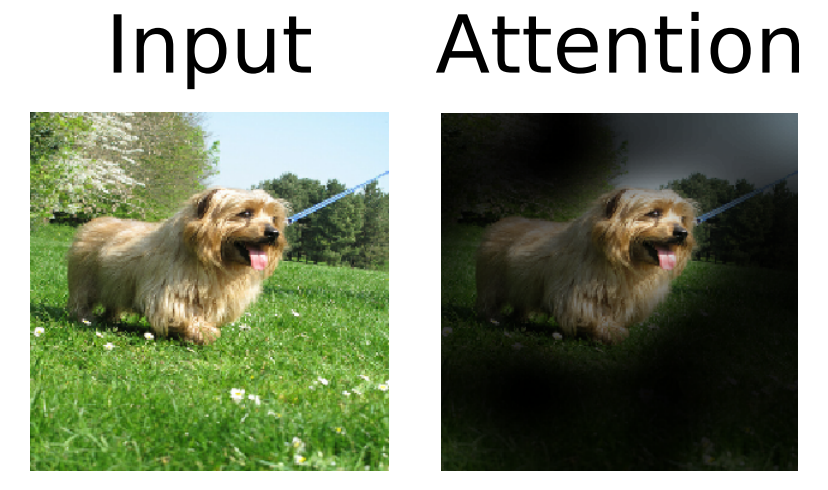
\includegraphics[scale=0.5]{res/vit-attention.png}
        \caption{Visualisation of self-attention for images in ViT \cite{dosovitskiy_image_2021}. Brighter pixels had greater importances computed between them by the transformer.}
        \label{fig:vit_attention}
    \end{figure}
    
    Other models have since built on ViT. Most significantly for segmentation, Pyramid Vision Transformer (PVT) \cite{wang_pyramid_2021} modifiers ViT to be more suitable for dense prediction, implementing $4 \times 4$ instead of $16 \times 16$ image patches for increased feature detail. To maintain performance (and develop multi-scale features), it then progressively merges patches between transformer blocks. DeIT \cite{touvron_training_2021} proposes a student-teacher and distilled training approach that allows ViT’s architecture to perform strongly even when pre-trained on far smaller datasets. Swin Transformer \cite{liu_swin_2021} builds hierarchical feature maps like PVT by merging image patches, but only computes self-attention within each window for efficiency. Twins \cite{chu_twins_2021} combines locally-grouped and global self-attention to achieve state-of-the-art performance.
    
    While CNNs need to gradually reduce image resolution to effectively increase receptive field, transformers have possess global attention. Significant relationships within the input sequence can be learned at all parts of the model regardless of their distance from one another. \cite{zheng_rethinking_2021} argues that this maintaining of resolution makes transformers especially suited for dense prediction. Their architecture, SETR, uses an encoder-decoder architecture with a pretrained traditional vision transformer (such as ViT or DeIT) as a backbone. Multiple decoders were assessed, with a progressive upsampling and convolution-based approach proving most effective. Most notably (as with ViT), it was found that backbone pre-training was essential. Without pre-training, SETR achieved only 42\% mIoU on Cityscapes, worse than models with 1\% the parameters \cite{paszke_enet_2016}. However, with pre-training, SETR achieved a state-of-the-art 82.15\% mIoU on Cityscapes. This is further evidence that, while ineffective with small data, vision transformers are capable of learning a far larger feature distribution and are therefore more transferable.
    
    SETR demonstrated the capacity of transformers in segmentation, but was limited by its use of a backbone designed for classification. SegFormer \cite{xie_segformer_2021} addressed a number of these issues using it’s Mix Transformer Encoder (MiT). First, dense $4 \times 4$ pixel patches and progressive patch merging are used as in PVT \cite{wang_pyramid_2021}. Rather than pure-MLP layers after each attention block, SegFormer employs MLPs mixed with $3 \times 3$ convolutions without zero-padding. This leaks spatial spatial information to the model that bypasses the need for positional encoding. Combined with a simple all-MLP encoder, possible due to the transformer’s receptive field, SegFormer achieves a state-of-the art 51.0\% mIoU on the new, challenging ADE20K dataset \cite{zhou_semantic_2018}.
    
    \subsection{Fast segmentation with transformers}
    Due to the success of transformer architectures in segmentation, recent research has explored the use of transformers for efficient, low-memory segmentation. Some approaches look to modify existing segmentation transformer architectures. \cite{bai_dynamically_2021} dynamically prunes the $Q$, $K$, and $V$ neurons of SegFormer’s \cite{xie_segformer_2021} parameters by removing all but the $r\%$ most activated. A knowledge distillation \cite{chen_learning_2017} approach is then used to bridge the gap between the original and pruned SegFormer. The un-pruned model becomes the ‘teacher’ and the pruned the ‘student’ - at each SegFormer block, the mean-squared error between the outputs of the student and teacher are added to the loss function.
    
    MobileViT \cite{mehta_mobilevit_2022} sought to modify the ViT architecture to reintroduce some of CNN's inductive biases and therefore reduce the parameters required for strong results. Rather than treating the input as a sequence of patch embeddings, MobileViT blocks take input and produce output as a $H \times W \times C$ tensor as CNNs do (figure ~\ref{fig:mobilevit_block}). This is then transformed to a ViT-like patch-embedding, where attention is applied along the size of the patches to avoid the loss of positional information that removes inductive bias. MobileViT was found to outperform MobileNetV2 across computer vision tasks. TopFormer \cite{zhang_topformer_2022} uses a U-Net-like \cite{ronneberger_u-net_2015} CNN-based encoder-decoder architecture where self-attention is applied only to the deepest features to minimise the required computation.
    
    \begin{figure}[ht!]
        \centering
        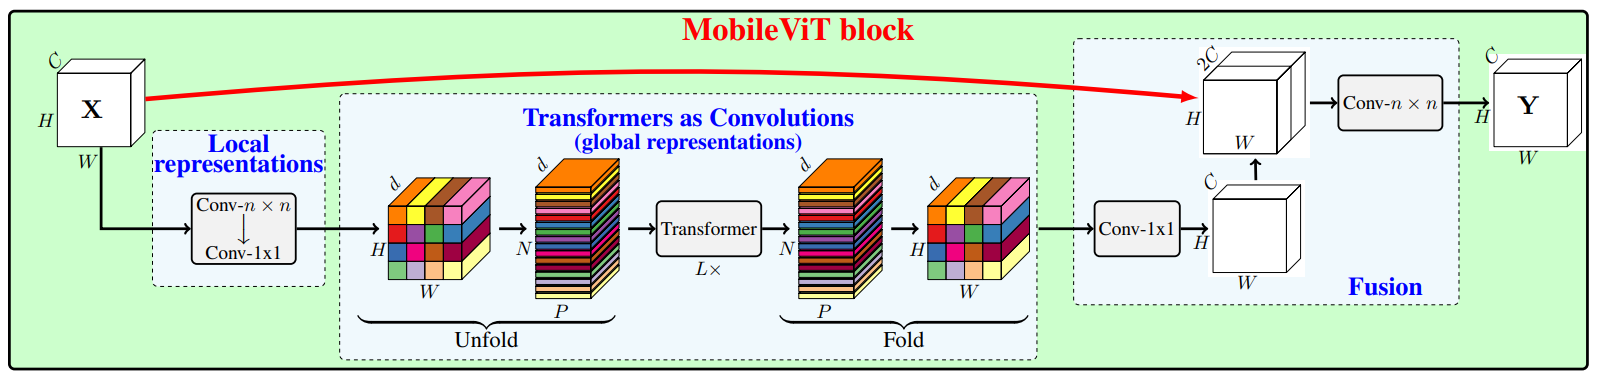
\includegraphics[width=\textwidth]{res/mobilevit-block.png}
        \caption{Architecture of a MobileViT block \cite{mehta_mobilevit_2022}. Features are input in CNN-like $H \times W \times C$ format, unfolded into a transformer input sequence, then re-folded into before being output.}
        \label{fig:mobilevit_block}
    \end{figure}
    
    \section{Domain adaptation}
    
    Domain adaptation is a diverse area of deep learning, as it seeks to address one of the greatest ongoing issues in the field - the lack of large amounts of high-quality training data for most tasks. Definitions of domain adaptation vary across literature, but in general, domain adaptation can be considered a subset of transfer learning: the transferring of learned knowledge about one domain to a new domain. To explain transfer learning, consider we are building a model to classify images with only a small amount of training data, which we denote the target dataset. We find our model cannot sufficiently learn high-level representations of the target dataset from the available training data, and will likely overfit to a local minima in the training set. However, if we first train the model on a much larger dataset such as ImageNet (denoted the source set), we will produce a model that has learned many features of the classes in this dataset, but also robust interpretations of common image features in general. If we initialise the model for training on the target set with the weights learned from the source set, we can intuit that the model will begin learning to classify the target set much closer to a global optimum for the task. This kind of transfer learning, using appropriate datasets, has been found to improve neural network performance almost universally \cite{sun_revisiting_2017}.
    
    Put more formally, consider the source dataset $D_S$ consisting of inputs $X_S$ and labels $Y_S$ as samples from an overall distribution $P_S$. Similarly, the target set $D_T$ consists of $X_T$ and $Y_T$ from a distribution $P_T$. Due to the domain shift between the datasets, we can intuit $P_T \neq P_S$. Therefore, transfer learning involves strategies for moving from $P_S$ to $P_T$ given our intuition $P_S$ will be a strong starting point for learning $P_T$. Domain adaptation, then, is an extension of this task where the target dataset's labels are not available \cite{wilson_survey_2020} - $Y_T$ is not known, making this an unsupervised learning problem.
    
    Domain Adaptation is an extremely common and practical problem in deep learning due to the high cost of labelling images for supervised training, especially in semantic segmentation. Each finely labelled image in the Cityscapes dataset, for instance, took human volunteers over 1.5 hours to produce on average \cite{cordts_cityscapes_2016}. Therefore, extensive research has been performed on the topic across all deep learning domains, including computer vision and semantic segmentation.
    
    Domain adaptation can massively improve the accessibility of domain adaptation. The majority of datasets for machine learning tasks, especially datasets with small and detailed labels like semantic segmentation \cite{cordts_cityscapes_2016} \cite{chen_semantic_2016} \cite{geiger_vision_2013}, are sourced from first-world countries where most machine learning research takes place. This means these demographics will disproportionately see the benefits of machine learning technologies. A self-driving car trained primarily on datasets from Europe and North America, for instance, would be prone to far more issues if operated without adjustment in other areas of the world. Domain adaptation makes it easier for research groups and demographics with less access to large datasets to see similar benefits, which can be safety-critical depending on the application.
    
    Another important distinction is between feature-level (i.e. domain-level) and label-level (i.e. task-level) adaptation. Feature-level is more common in domain adaptation, which is simply where the source and target distributions differ ($P_T \neq P_S$) \cite{wilson_survey_2020}. Label-level adaptation has the set of labels to apply to the source and target dataset differ - a problem that requires vastly different approaches. This review discusses research into feature-level domain adaptation.
    
    \subsection{Domain adaptation approaches in deep learning}
    
    Many approaches have been proposed for transferring strong predictive power from a source domain to an unlabeled target domain. A large subset of strategies focus on aligning the feature space between the source and target dataset - if a model trained on the source set can produce similar features on the target set, we intuit it will likely be better at classifying/decoding these features for the target domain.
    
    One approach to this is “domain invariant feature learning” \cite{wilson_survey_2020} - explicitly encouraging the model encoder to produce similar feature representations for source and target inputs by adding a new component to the loss. Some approaches compute difference as the distance between the distributions of the features. This can be evaluated through metrics like maximum mean discrepancy (MMD) \cite{gretton_kernel_2006} or correlation alignment (CORAL) \cite{sun_return_2015}. \cite{rozantsev_beyond_2019}, for instance, produce a model with two parallel streams (for source/target data respectively), and employ MMD between extracted features in the loss to adapt from synthetic to real drone detection data.
    
    Recently, many approaches have applied adversarial approaches to domain invariant feature learning. Adversarial networks \cite{goodfellow_generative_2014} are a subclass of deep neural networks that make two models compete in a zero-sum game. In a typical scenario, a generator model will produce outputs in an attempt to 'trick' a discriminator, which takes in the generator’s output, into making the wrong prediction. The performance of each model is then used to negatively affect the other’s loss - both attempt to minimise the performance of the other. A common example is the creation of artificial faces \cite{karras_progressive_2018} - the generator produces artificial faces, while the discriminator takes in images and attempts to classify whether they are real or produced by the generator. Both models then compete against each other in alternate training until convincing face generation is achieved. \cite{ganin_domain-adversarial_2016} employ an adversarial discriminator model applied to a model’s encoder output, which tries to distinguish whether the features were produced from the source or target distribution. This model’s performance is then added to the main model loss (via gradient reversal), encouraging the model to produce source and target domain features that are indistinguishable from one another.
     
     \begin{figure}[t]
        \centering
        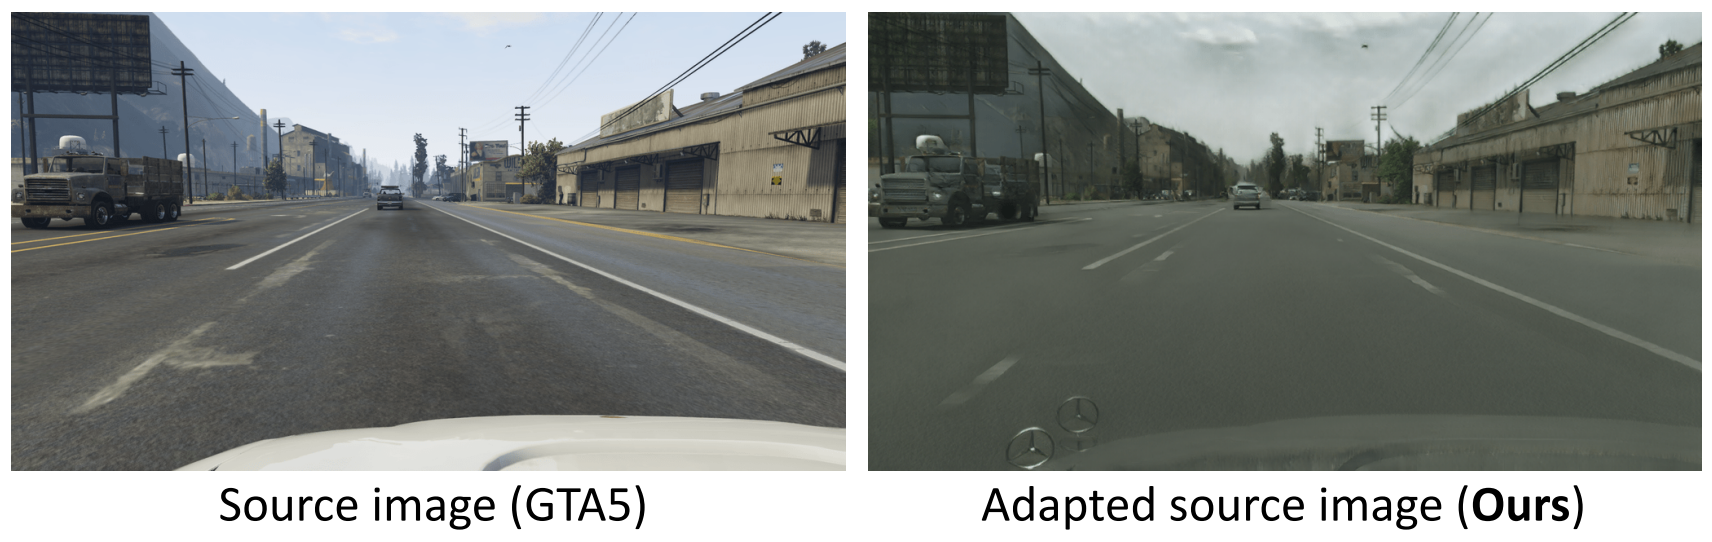
\includegraphics[width=\textwidth]{res/cycada-example.png}
        \caption{An example of GTA5 \cite{richter_playing_2016} to Cityscapes \cite{cordts_cityscapes_2016} domain adaptation using CyCADA \cite{hoffman_cycada_2017}.}
        \label{fig:cycada_example}
    \end{figure}
    
    Other approaches move domain invariance a step backwards by adapting the labelled source input images themselves to cross the domain gap and match the target distribution \cite{wilson_survey_2020} (figure ~\ref{fig:cycada_example}). This is most commonly achieved using GANs \cite{mirza_conditional_2014} \cite{hoffman_cycada_2017}. Alternatively, training can be done on labelled source images transferred to match the target distribution for inference on the unmodified target distribution images. A key assumption in this approach is that the differences in the source/target domain are low-level \cite{wilson_survey_2020}.

    Pseudo-labelling \cite{wilson_survey_2020}, sometimes called transductive learning \cite{kamnitsas_transductive_2021}, is another core approach. It is based on the idea that the highest quality/most “confident” predictions on the unlabelled target data will provide more valuable than non-valuable knowledge to the model. \cite{kamnitsas_transductive_2021} analyse this in the context of information gain - given an appropriate confidence, choosing the $r\%$ most confident predictions on the target set and adding these to the training set will provide positive information gain. Whether a prediction is considered ‘confident’ can be determined by using an ensemble of diverse models. If a prediction is consistent in a high proportion of the ensemble, we can intuit it is more likely to be correct. Many approaches, especially in semantic segmentation however, instead assume that the magnitude of a model’s softmax prediction can be used as a measure of confidence and therefore pseudo-labelling \cite{zou_domain_2018}. Recent classification approaches such as SHOT \cite{liang_we_2021} instead produce pseudo-labels via k-means clustering followed by k-nearest neighbours classification on the zero-shot \cite{larochelle_zero-data_2008} target dataset predictions, and achieve state-of-the-art results.
    
    Many authors combine a number of the above and other approaches. Target discriminative approaches, for instance, take advantage of the cluster assumption \cite{chapelle_semi-supervised_2005}, which states that features with common labels should be clustered together in the feature space. Therefore, class boundaries should lie in the low density regions between clusters. Numerous adversarial approaches have been explored to move the decision boundary into these low-density regions \cite{wilson_survey_2020}.
    
    \subsection{Domain adaptation for semantic segmentation}
    
    As a task with especially challenging label production \cite{cordts_cityscapes_2016}, domain adaptation for semantic segmentation has been explored extensively in recent years. Many approaches focus on adaptation from far more easily attainable synthetic segmentation datasets (such as GTA5 \cite{richter_playing_2016} and SYNTHIA \cite{ros_synthia_2016}) to real-world datasets (such as Cityscapes \cite{cordts_cityscapes_2016}, where labels are considered missing and only used for benchmarking).
    
    As with general semantic segmentation, many developments for segmentation DA are adapted and inspired from developments in simpler computer vision tasks. Approaches described in the previous section have been applied to the semantic segmentation task in various forms. However, early approaches found domain adaptation for segmentation is far more challenging due to the increased complexity and scale of the task \cite{csurka_unsupervised_2021}. Using FCN, \cite{hoffman_fcns_2016} addresses these issues by learning from both a pixel-wise domain discriminator loss and a class-wise discriminator loss as multiple classes will likely be present in each prediction. This work is often considered the earliest domain adaptation approach segmentation. Another U-Net \cite{ronneberger_u-net_2015} based approach \cite{bermudez-chacon_domain-adaptive_2018} applies MMD at multiple upsample layers across the model to adapt the denser representations. DANNet \cite{wu_dannet_2021} applies adversarial discriminator loss directly to the output predictions of target domain day-night images. \cite{benjdira_unsupervised_2019} apply GAN-based image translation to aerial images to achieve significant improvements in segmentation performance. However, even with these more advanced approaches, the success of pure domain alignment for semantic segmentation has been limited.
    
    Much greater success has been found with pseudo-labelling strategies, which are a common feature of many recent state-of-the art segmentation domain adaptation approaches. In their highly influential work, \cite{zou_domain_2018} make a number of contributions. First, the concept of pseudo-labeling is extended to semantic segmentation - the magnitude of softmax score is considered as the prediction confidence for each pixel. After each epoch, all target set images are added to the training set as pseudo-labels, though all but the $r\%$ most confident of all pixel predictions are “masked out” (made to not influence training) (figure ~\ref{fig:cbst_overview}). Intuiting that the model’s target set performance will initially be poor, a scheduling system is introduced where $r$ starts low and is gradually increased as the model improves. \cite{kamnitsas_transductive_2021} use ensembles to better estimate model confidence, finding underconfident models provide much more information to the task. \cite{zou_domain_2018} also introduces class-balancing: given predictions in segmentation need to be made for multiple classes on each image, we can presume some classes will have a smaller domain gap between $D_S$ and $D_T$. For instance, for a road-scene labelling task, roads between the two datasets may be highly similar while cars are highly different. Therefore, simply choosing the $r\%$ highest-confidence predictions for pseudo-labels would likely make the model choose only easy-to-adapt classes as pseudo-labels and ignore difficult classes, which would only get worse as training continues. Therefore, predictions are normalised per-class, with the top $r_c\%$ (for class $c$) predictions then chosen per-class. Finally, the concept of spatial priors is introduced - the average frequency of each class at a given location in the source dataset is used to modify the confidence of target dataset predictions for pseudo-labelling, encouraging pseudo-labels with a similar distribution (e.g. sky is more likely to appear at the top of the image, and should be encouraged). 
    
    \begin{figure}[t]
        \centering
        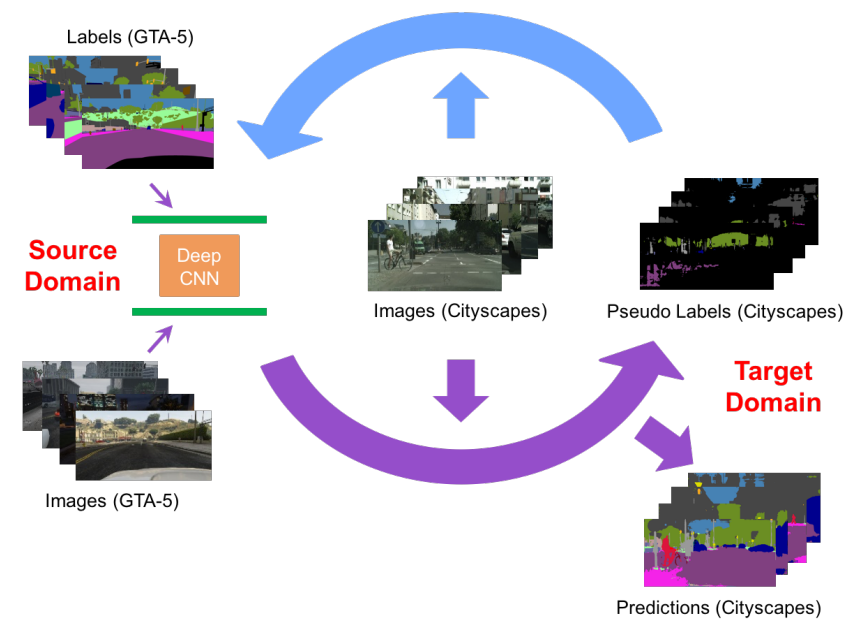
\includegraphics[scale=0.7]{res/cbst-overview.png}
        \caption{An overview of the class-balanced self-training (CBST) pipeline \cite{zou_domain_2018}.}
        \label{fig:cbst_overview}
    \end{figure}

    CBST’s have been widely adopted across fields of domain adaptation, though not all agreement has been universal. ADVENT \cite{vu_advent_2019} actually found training on low-confidence regions to boost performance. Based on the observation that source set predictions are often overconfident (low-entropy) and target underconfident (high-entropy), it’s approach focuses on minimising model entropy using an adversarial loss. \cite{li_bidirectional_2019} combines GAN image translation with pseudo-labelling through bidirectional learning. After initial training of a segmentor and a $X_S$ to $X_T$ GAN, pseudo label predictions are made, and the most confident labels are both (a) fed into the training set and (b) used to re-train the GAN, improving its ability to support crossing the domain gap. \cite{wang_differential_2020} also explores challenge of aligning different image subsets in segmentation, denoting the alignment difference between stuff (background image content like roads) and things (instance based content like cars). While stuff classes can often be aligned globally between datasets, instances of things may differ in distribution even within a single source image. Therefore, separate adversarial losses are applied for each - one for global stuff alignment and one for instance-based thing alignment. Ultimately, adversarial loss and pseudo-label loss have become the primary approaches for domain alignment for semantic segmentation and general computer vision.
    
    \subsection{Domain adaptation for vision transformers}
    
    The application of transformer networks to domain adaptation is a new and highly promising field. In many domains, transformers have also been widely adopted due to their strong transfer learning capabilities \cite{radford_language_2019} \cite{wright_transformer_2020}. The same applies for vision - as explored by ViT \cite{dosovitskiy_image_2021} and SETR \cite{zheng_rethinking_2021}, transformers are very good at learning overall distributions through pre-training and then adapting to new labelled data.
    
    Many initial domain adaptation approaches applied transformers tangentially or to non-computer vision fields. \cite{shakeri_end--end_2020} apply transformers for text generation in NLP domain adaptation. \cite{liu_multi-task_2019} find training models on multiple NLP tasks results in improved domain adaptation performance over typical pre-training. \cite{yang_transformer-based_2021} apply a transformer after traditional CNN-based computer vision feature extractors to improve source-free domain adaptation by applying focus on relevant input object features. 
    
    TVT \cite{yang_tvt_2021} explores vision transformer’s general ability to perform domain adaptation. Surprisingly, ViT’s zero-shot transferability was found to outperform many state-of-the art techniques for classification domain adaptation. On the Office-31 \cite{saenko_adapting_2010} domain adaptation dataset, an ImageNet-pre-trained ViT achieves 81.45\%, a 7\% accuracy increase over SHOT \cite{liang_we_2021}. Multiple domain adaptation modifications were evaluated for TVT. Applying an adversarial domain discriminator on class token output (equivalent to CNN features) provided some improvements. Best results were seen by applying a patch-wise discriminator that de-emphasises patch weights that are easily discriminated, combined with a loss that maximises feature clustering \cite{chapelle_semi-supervised_2005}. \cite{wang_exploring_2021} similarly explore an original transformer architecture for object detection domain adaptation, applying adversarial feature alignment on each input patch.
    
    \begin{table}[t]
        \centering
        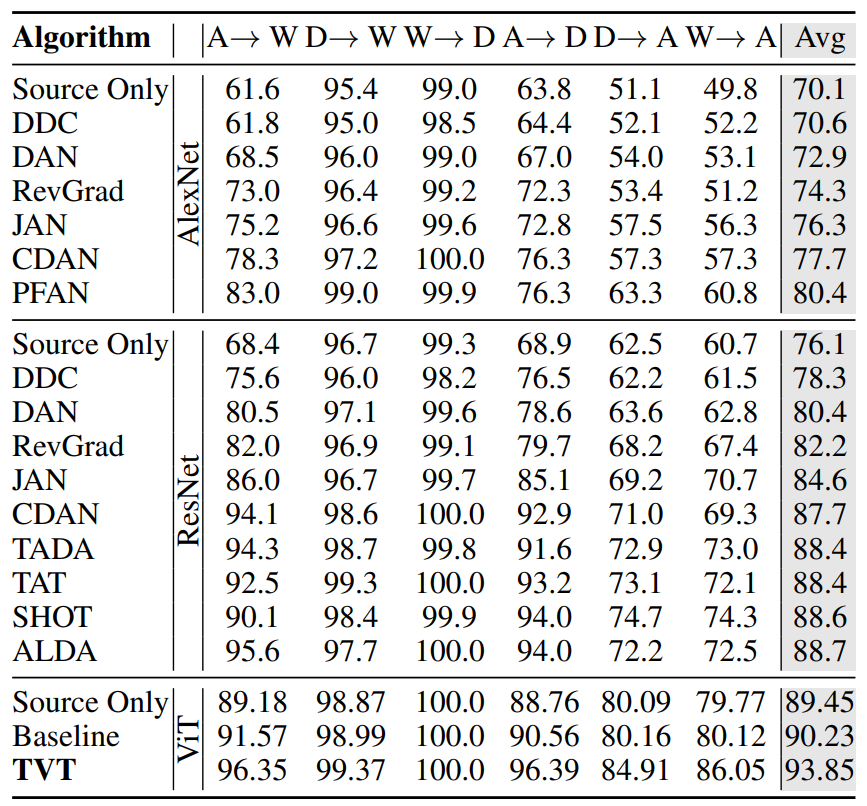
\includegraphics[scale=0.5]{res/vit-table.png}
        \caption{Performance comparison of TVT against other domain adaptation approaches \cite{yang_tvt_2021}. Note the "Source Only" TVT model (bottom row) consistently outperforms CNN-based domain adaptation approaches with access to the source data.}
        \label{tab:vit_table}
    \end{table}
    
   \begin{figure}[ht]
        \centering
        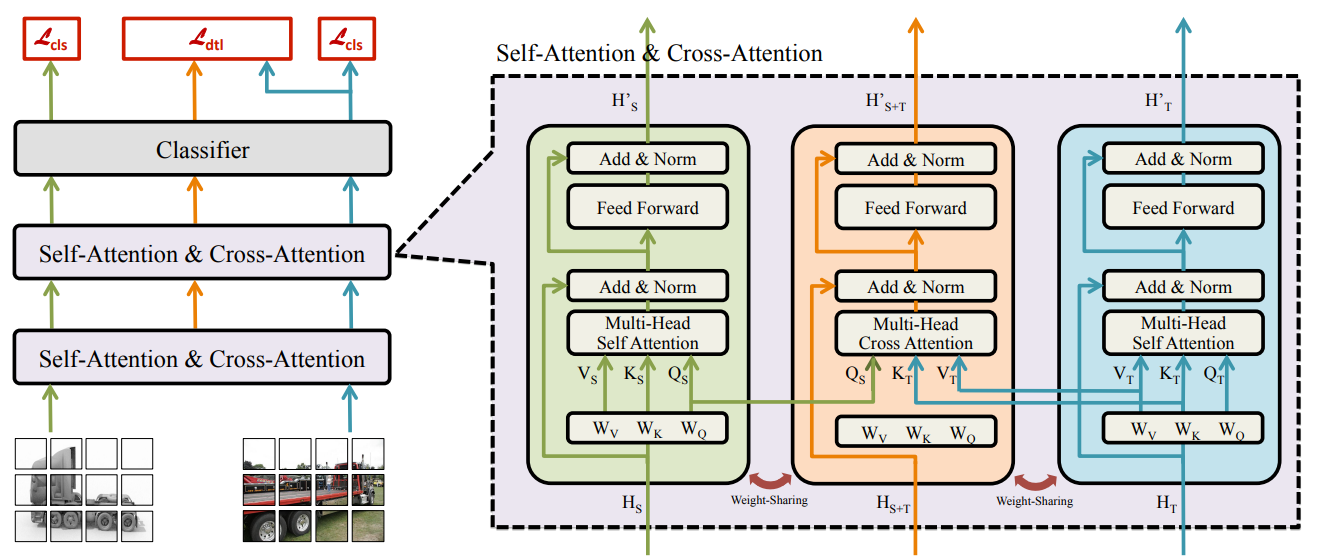
\includegraphics[width=\textwidth]{res/cdtrans-architecture.png}
        \caption{Architecture of CDTrans \cite{xu_cdtrans_2021}. The source-target branch (centre) receives output from the source branch's $Q$ and the target branch's $K$ and $V$ values.}
        \label{fig:cdtrans_architecture}
    \end{figure}
    
    Transformers, specifically cross-attention, have been found to be effective in tasks that require crossing even extremely large task or domain gaps. Cross-attention has successfully been used to learn inter-image feature extraction \cite{li_trear_2021}  and even image-to-text speech alignment \cite{tsai_multimodal_2019}. CDTrans \cite{xu_cdtrans_2021} applies a pseudo-labelling approach as in SHOT \cite{liang_we_2021} to take advantage of this for domain adaptation. It uses 3 ViT-like backbone branches - source, target, and source-target - all with shared weights (figure ~\ref{fig:cdtrans_architecture}). The source and target branches take in similar images from the source and target sets respectively, and compute self-attention on them. The source-target branch then computes cross-attention between the outputs at each block. The intuition behind this is that if false pseudo-labels are given (the main drawback of pseudo-labelling), cross attention will assign low weights to the dissimilar features produced, which will mitigate the backpropagation effects of these blocks. The output of cross-attention (which should possess the most domain-invariant features) is then used to make a prediction on the target, and the result’s difference to the target branch output is added to the loss to encourage learning-cross domain features (and minimise the effect of false positives). Once domain-invariant feature extraction is learned throughout the network, only the target branch is used for inference.

    The idea of using cross-attention is extended in BCAT (Bi-Directional Cross-Attention Transformer) \cite{wang_domain_2022} which introduces a target-source branch alongside the source-target branch that computes cross-attention on the source rather than the target data (figure ~\ref{fig:bcat_block}). Instead of CDTrans’ student-teacher approach, an MMD transfer loss is then between the merged feature outputs of the target/source-target branch and the source/target-source branch (figure ~\ref{fig:bcat_architecture}). This approach maintains the benefit of cross-attention in terms of false-positive pseudo-labels while more directly encouraging the learning of domain-invariant features.
    
    \begin{figure}
        \centering
        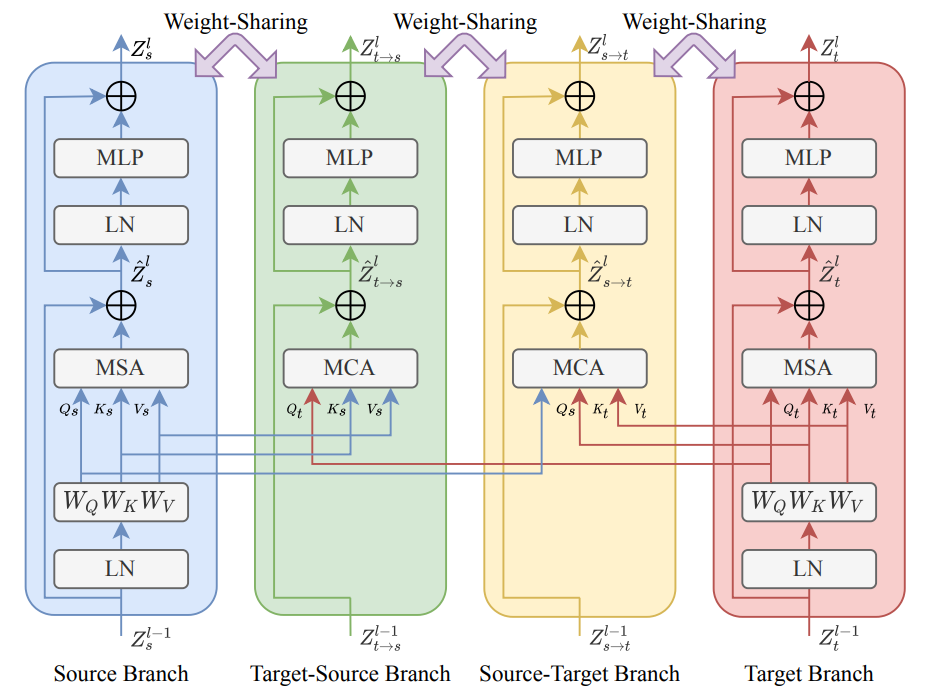
\includegraphics[width=\textwidth]{res/bcat-block.png}
        \caption{Structure of BCAT block \cite{wang_domain_2022}.}
        \label{fig:bcat_block}
    \end{figure}
    \begin{figure}
        \centering
        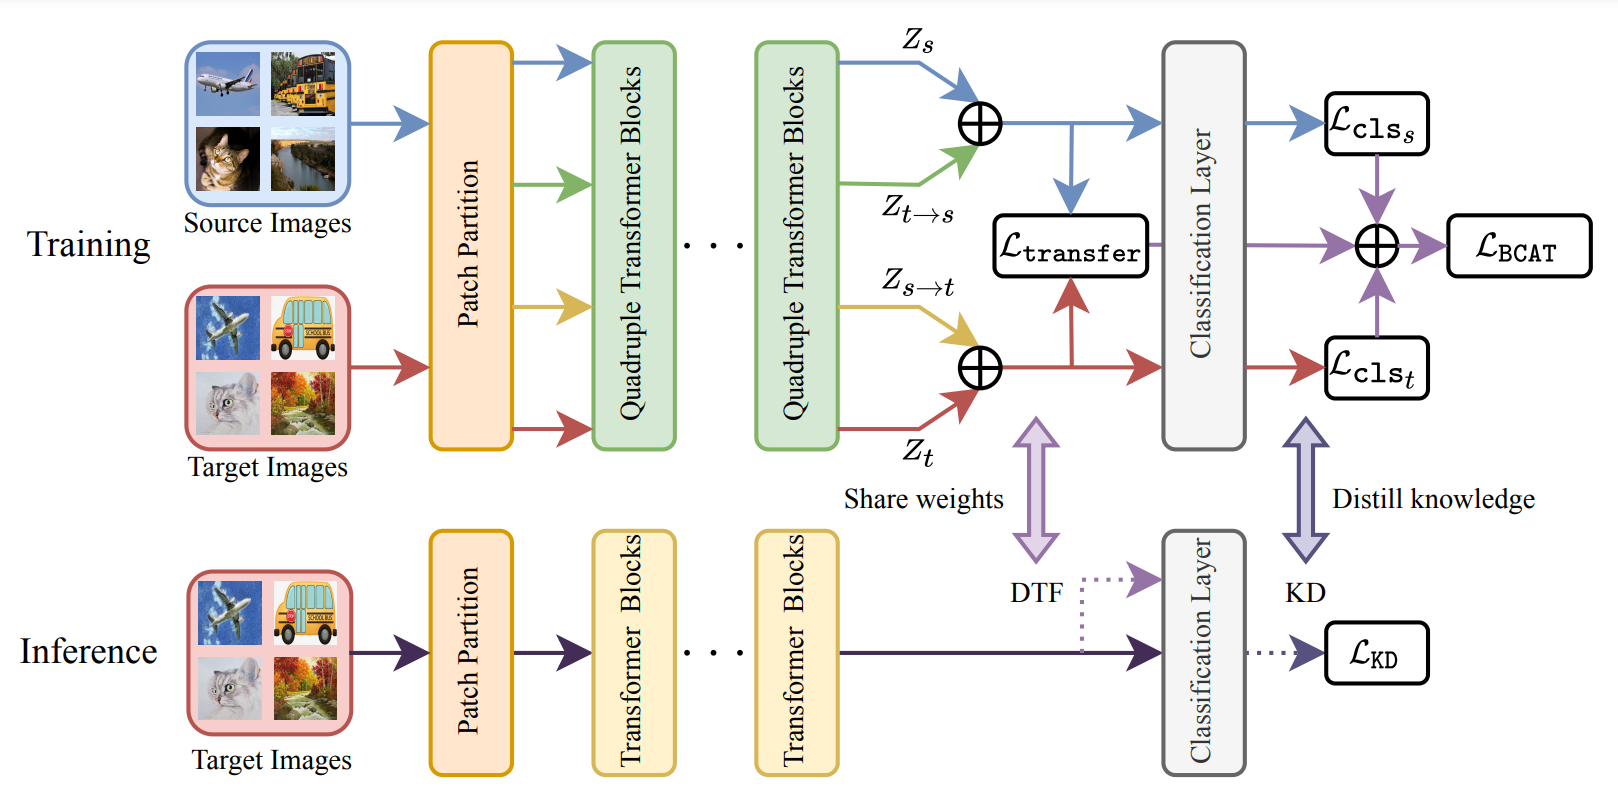
\includegraphics[width=\textwidth]{res/bcat-architecture.png}
        \caption{Overall BCAT architecture \cite{wang_domain_2022}. Transfer loss is computed between the fused source/target source and target/source-target features, then added to overall loss.}
        \label{fig:bcat_architecture}
    \end{figure}

    Despite the recent promising results achieved using segmentation transformers and the established strong domain adaptation abilities of transformers in computer vision, only one publication (at the time of writing) has explored transformer domain adaptation for semantic segmentation. DTNet \cite{li_dispensed_2021} focuses on the medical segmentation. The architecture improves the efficiency of multi-head-self-attention by applying attention separately on a channel-wise, neighbour-wise, and dilated basis. This is combined with a patch-wise domain discriminator similar to \cite{yang_tvt_2021} to prioritise transferable features. Therefore, there exists an opportunity to apply other transformer-specific domain adaptation approaches \cite{yang_tvt_2021} \cite{xu_cdtrans_2021} \cite{wang_domain_2022} to semantic segmentation with appropriate architectural modifications.

\bibliographystyle{IEEEtran}
\bibliography{lit-review}

\end{document}